\documentclass[12pt]{article}
\usepackage[swedish]{babel}
\usepackage[version=4]{mhchem}
\usepackage{amsmath}
\usepackage[swedish]{varioref}
\usepackage{hyperref}
\hypersetup{
    colorlinks=true,
    linkcolor=black
}
\usepackage[swedish]{cleveref}
\usepackage{amsthm}
\usepackage{cancel}
\usepackage{float}
\usepackage{array}
\usepackage{enumitem}
\renewcommand{\labelitemii}{$\circ$}

\makeatletter
  \@addtoreset{section}{part}
\makeatother 

\theoremstyle{definition}
\newtheorem{exm}{Exempel}

\title{Begreppssammanfattning - Kemi 2 \\ Blackebergs Gymnasium}
\author{Marcell Ziegler - NA21D}

\begin{document}
    \begin{titlepage}
        \maketitle
        \vfill
        
        \begin{center}
            \textbf{OBS!} Alla siffror/refenser som verkar/borde vara länkar är \\ antagligen länkar, tryck gärna!
        \end{center}
    \end{titlepage}

    \tableofcontents

    \newpage

    \part{Kemisk jämvikt}
    
    En jämvikt är en kemisk reaktion som går åt båda håll med samma reaktionshastighet (lika snabbt). Detta medför att förhållandet mellan reaktanter och produkter förblir densamma. Egentligen är alla reaktioner jämvikter men vissa är så pass förskjutna åt ena hållet att de betraktas som fullständiga. Tecknet $\ce{<=>}$ används för att visa jämvikt, se följande exempel:
    \begin{equation*}
        \ce{HCl + H2O <=> H3O+ + Cl-}
    \end{equation*}

    \section{Jämviktskonstanten}

Varje kemisk jämvikt har en s.k. jämviktskonstant $K$. Detta beräknas enligt denna formel\footnote{Se s. 42--48 samt uppgift 3:1--3:3} ($n_{prod} = \text{antal produkter och } n_{reakt} = \text{antal reaktanter}$):
\begin{gather*}
    \label{eq:jmvkonstant}
    K = \frac{\prod_{n=1}^{n_{prod}}[\mathrm{produkt}_n]}{\prod_{n=1}^{n_{reakt}}[\mathrm{reaktant}_n]} \\
    \text{alltså\ldots} \\
    K = \frac{[\mathrm{produkt}_1] \cdot [\mathrm{produkt}_2] \dotsm [\mathrm{produkt}_{n_{prod}}]}{[\mathrm{reaktant}_1] \cdot [\mathrm{reaktant}_2] \dotsm [\mathrm{reaktant}_{n_{reakt}}]}
\end{gather*}
$K$ visar alltså förhållandet mellan produkterna av koncentrationerna av produkter och reaktanter. Detta leder även till dessa två till slutsatser:
\begin{align*}
    \text{större } K \Rightarrow \text{mindre reakt. eller mer prod. i jämförelse} \\
    \text{mindre } K \Rightarrow \text{mer reakt. eller mindre prod. i jämförelse} 
\end{align*}
\pagebreak
\begin{exm}
    Vid jämvikt finns det $ \mathrm{0.045\,M} \ \ce{H2O},\ \mathrm{0.005\,M} \ \ce{H2} \text{ och } \mathrm{0.0025\,M} \ \ce{O2}$ i reaktionen
    \begin{equation*}
        \ce{2H2O <=> 2H2 + O2}
    \end{equation*}
    Sätter man in siffrorna får man
    \begin{equation*}
        K = \frac{\mathrm{[H_2O]^2 \cdot [O_2]}}{\mathrm{[H_2O]^2}} \approx 2.78 \cdot 10^{-4} \, \mathrm{M}
    \end{equation*}
    Lägg märke till att vissa koncentrationer är upphöjda till en exponent. Denna exponent är alltid samma som ämnets koefficient i reaktionen. \\ $\ce{2H2O \rightarrow [H2O]^2}$ exempelvis.
\end{exm}

\subsection{Enheten på \textit{K}}

Detta beräknas med en enhetsanalys på koncentrationerna\footnote{Se uppgift 3:4}.

\begin{exm}
    Givet situationen från ovan, sätt in enheter:
    \begin{equation*}
        K \approx 2.78 \cdot 10^{-4} \mathrm{ \left[\frac{M^2 \cdot M}{M^2} = \frac{M^{\cancelto{1}{3}}}{M^{\cancel{2}}} = M\right]}
    \end{equation*}
\end{exm}

\subsection{Räkna på \textit{K}}

Du ska kunna räkna ut $K$ för en viss reaktion utifrån ett fåtal substansmängder eller koncentrationer\footnote{Se s. 48--49 samt uppgift 3:7}.

\begin{exm}
    Titta på exemplet i denna tabell ($C_0$ är koncentration från början och $C_{jmv}$ är koncentration vid jmv.):
    
    \begin{table}[H]
        \centering
        \begin{tabular}{|c|c|>{\centering\arraybackslash}m{31.5pt}|c|} 
        \cline{2-4}
        \multicolumn{1}{l|}{} & \multicolumn{3}{c|}{$\ce{\hspace{7pt} A \hspace{7pt} + \hspace{7pt} B \hspace{2pt} <=> \hspace{2pt} AB} \hspace{15pt}$}  \\ 
        \hline
        $C_0$                 & $x$   & $x$   & $0$                       \\ 
        \hline
        $\Delta C$            & $-y$  & $-y$  & $+y$                      \\ 
        \hline
        $C_{jmv}$             & $x-y$ & $x-y$ & $y$                       \\
        \hline
        \end{tabular}
    \end{table}
    
    \noindent vilket ger att
    
    \begin{equation*}
        K = \frac{[\mathrm{AB}]}{\mathrm{[A] \cdot [B]}} = \frac{y}{(x-y)^2} \, \mathrm{\left[\frac{M}{M^2}=M^{-1}\right]}
    \end{equation*}
    
    Notera att förhållendet mellan $\Delta C$ hos de olika ämnen är densamma som deras koefficient i rekationen så följande gäller i mer komplexa fall:
    
    \begin{table}[H]
        \centering
        \begin{tabular}{|c|c|>{\centering\arraybackslash}m{31.5pt}|c|} 
        \cline{2-4}
        \multicolumn{1}{l|}{} & \multicolumn{3}{c|}{$\ce{\hspace{10pt} 2A \hspace{7pt} + \hspace{9pt} B \hspace{1.5pt} <=> \hspace{2pt} A2B} \hspace{15pt}$}  \\ 
        \hline
        $C_0$                 & $z$   & $x$   & $0$                       \\ 
        \hline
        $\Delta C$            & $-2y$  & $-y$  & $+y$                      \\ 
        \hline
        $C_{jmv}$             & $z-2y$ & $x-y$ & $y$                       \\
        \hline
        \end{tabular}
    \end{table}
    
    \begin{equation*}
        K = \frac{[\mathrm{AB}]}{\mathrm{[A] \cdot [B]}} = \frac{y}{(z-2y) \cdot (x-y)} \, \mathrm{\left[\frac{M}{M^2}=M^{-1}\right]}
    \end{equation*}
\end{exm}
    \setcounter{exm}{0}
    \section{Förskjutning av reaktioner}

I uppgifter behöver man ofta bestämma hur en rekation kommer \emph{förskjutas} eller vilket håll den kommer ''gå mot''. Alla jämvikter vill till slut uppnå det jämviktsförhållande som är givet av deras $K$-värde under givna förhållanden. Om man börjar från ett tillstånd utan jämvikt eller om jämvikten rubbas kommer reaktionen att förskjutas. Detta innebär att antingen mängden reaktanter eller produkter kommer öka eller minska. När antalet produkter ökar jämfört med reaktanterna kallas det att reaktionen förskjuts åt höger och motsatsen kallas förskjutning åt vänster.

\subsection{Reaktionskvoten}

Förhållandet mellan produkter och reaktanter när det inte råder jämvikt beskrivs av \emph{reaktionskvoten} $Q$. Formeln för $Q$ är exakt samma som för $K$. Vid jämvikt är $Q=K$ men övrigt så är den antingen större eller mindre. Det finns två enkla regler angående $Q$-värdet:
\begin{align*}
    &Q > K \Rightarrow \text{fler produkter eller färre reaktanter} \Rightarrow \\ 
    &\Rightarrow \text{förskjutning åt vänster} \\
    &Q < K \Rightarrow \text{färre produkter eller fler reaktanter} \Rightarrow \\ 
    &\Rightarrow \text{förskjutning åt höger}
\end{align*}

\subsection{Tillskott av ämnen}
\subsubsection[Reaktanter]{Tilskott av reaktanter}
Om det finns en reaktion i jämvikt och fler reaktanter läggs till kommer $\prod^{n_{reakt}}_{n=1}[\mathrm{reaktant}_n]$ öka vilket innebär att $Q$ kommer minska (se \cref{eq:jmvkonstant}). Enligt definitionen ovan kommer reaktionen gå åt höger.
\subsubsection[Produkter]{Tillskott av produkter}
Om en reaktion i jämvikt får ett tillskott av produkter kommer $\prod^{n_{prod}}_{n=1}[\mathrm{produkt}_n]$ att öka vilket innebär att $Q$ kommer öka (se \cref{eq:jmvkonstant}). Enligt definitionen ovan kommer reaktionen gå åt vänster.
    \setcounter{exm}{0}

    \pagebreak

    \part{Reaktionshastighet}

    Reaktionshastighet är en annan central del av denna kurs. Kortfattat är det hur snabbt en reaktion sker uttryckt i $\mathrm{\left[\frac{Molar}{Sekund} = \frac{M}{s} = \frac{mol}{dm^3 \cdot s}\right]}$. Detta ger oss formeln 
    \begin{equation*}
        v = \frac{\Delta C}{\Delta t} 
    \end{equation*}
    där $v = \text{reaktionshastighet i } \mathrm{M/s}$. Om man av någon anledning hade velat teckna en funktion hade $v = C'(t) = \frac{dC}{dt}$ gällt.

    \section{Påverkande faktorer}
Reaktionshastigheten kan påverkars av många faktorer\footnote{se s. 28--31 i boken}. Här kommer en sammafattning.
\subsection{Bindningar}
Fria joner reagerar nästa omedelbart, exempelvis i fällningar. När detta sker är reaktionen \emph{momentan}. Fria joner har inte några bindningar som måste brytas innan reaktionen kan ske vilket gör det snabbare. Molekyler kommer alltid att reagera långsammare då det tar tid och energi att bryta deras bindningar för reaktionen.

\subsection{Kontaktyta}
Jo större ytan som reaktionen sker på är desto snabbare kommmer den att gå. Detta beror på att de reagerande ämnena måste kollidera för att reaktionen ska ske. Ju mer yta att kollidera på desto fler kollisioner alltså desto snabbare reaktion.

\subsection{Aggregationstillstånd}
Aggregationstillståndet, eller i detta fall hur fritt partiklarna rör sig, kommer ha en stor effekt på reaktionshastigheten. En gas kommer ju ha högst rörlighet, sedan vätskor och sist fasta ämnen. Ju mer partiklarna rör sig desto fler chanser kommer de få att kollidera med varandra och desto snabbare kommer reaktionen att gå.

\subsection{Katalysatorer}
\label{sec:katalysator}
En katalysator är ett ämne som gör en reaktion snabbare eller möjliggör en reaktion som annars är omöjlig utan att själv förbrukas. Den gör detta genom att sänka aktiveringsenergin (se \vref{sec:entalpiaktiveringse}) av reaktionen. Antingen kommer den att hamna under gränsen för tillgänglig energi vilket möjliggör reaktionen eller så kommer den helt enkelt minska energikravet och öka hastigheten.

\subsection{Koncentration}
En högre koncentration gör partiklarna tätare vilket i sin tur leder till snabbare reaktioner. Detta medför också att tryckförändringar påverkar reaktionshastighet i komprimerbar materia (ex. gaser).

\section{Reaktionens energi}

\subsection{Endoterm och exoterm}
\label{sec:endoexo}
En reaktion kan vara endo- eller exoterm. En endoterm reaktion kräver energi medan en exoterm reaktion avger ett överskott av energi\footnote{se s. 32--33 i boken}.

\subsection{Entalpi och aktiveringsenergi}
\label{sec:entalpiaktiveringse}
\begin{figure*}[h]
    \centering
    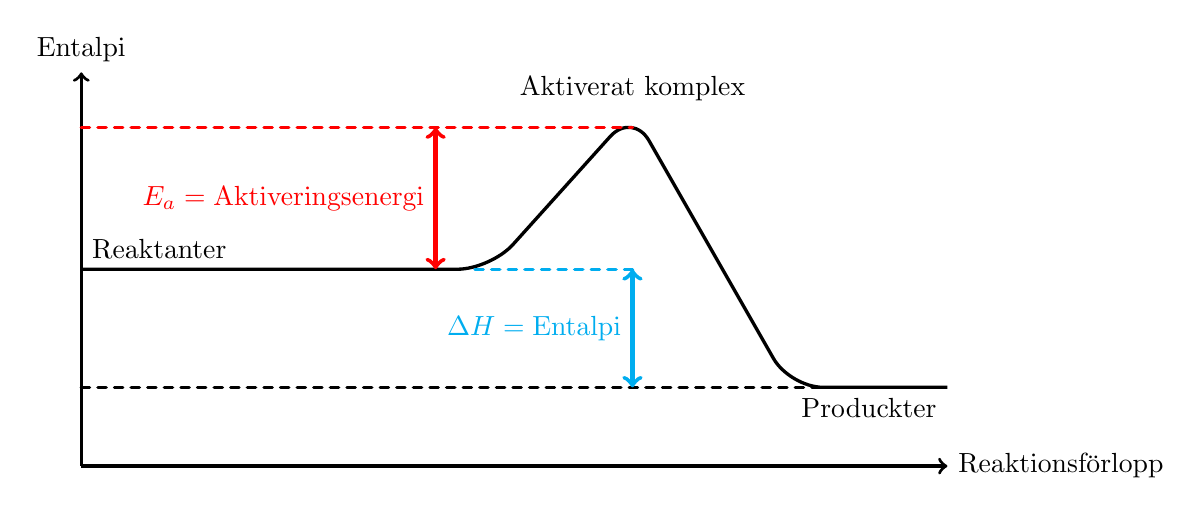
\begin{tikzpicture}
        \draw [->,very thick] (0,0) -- (0,5) node[anchor=south] {Entalpi};
        \draw [->,very thick] (0,0) -- (11,0) node[anchor=west] {Reaktionsförlopp};
        \draw [very thick,rounded corners=12pt] (0,2.5) node[anchor=south west] {Reaktanter} -- (5.2,2.5) -- (7, 4.5) node[anchor=south] {Aktiverat komplex} -- (9,1) -- (11,1) node[anchor=north east] {Produckter};
        \draw [dashed,very thick,color=red, line cap=round] (0,4.3) -- (7,4.3);
        \draw [dashed,very thick, line cap=round] (0,1) -- (10.5,1);
        \draw [ultra thick,<->,color=red] (4.5,2.5) -- (4.5,3.4) node[anchor=east] {$E_a = \text{Aktiveringsenergi}$} -- (4.5,4.3);
        \draw [very thick, dashed, color=cyan, line cap=round] (5,2.5) -- (7,2.5);
        \draw [ultra thick, <->, color=cyan] (7,1) -- (7,1.75) node[anchor=east] {$\Delta H =\text{Entalpi}$} -- (7,2.5);
    \end{tikzpicture}
\end{figure*}

\noindent Denna graf visar förloppet av en reaktion uttryckt som energiförändring över tid. Energin är mätt i enheten $\mathrm{kJ/mol}$ som på sätt och vis uttrycker energikoncentration baserat på substansmängd vilket kallas \emph{entalpi}\footnote{se s. 32--36 samt uppgift 2:11 i boken}. När man säger entalpi menar man ofta förändringen i entalpi som uttrycks $\Delta H$. Detta visar om det har avgetts eller absorberats energi under reaktionens gång:
\begin{align*}
    \Delta H < 0 &\Rightarrow \text{exoterm reaktion, energi avges} \\
    \Delta H > 0 &\Rightarrow \text{endoterm reatkion, energi absorberas}
\end{align*}

På grafen kan vi även den så kallade \emph{aktiveringsenergin} $E_a$. Denna energi är är skillnaden mellan den ursprungliga energinivån av reaktanterna och den mängd energi som krävs för att reaktionen ska ske. Man kan resonera kring aktiveringsenergi från båda hållen i diagrammet. Just nu finns bara det högra hållet inritat, men i jämvikter går ju det åt båda håll och därmed finns det värde även i produkt $\rightarrow$ reaktant resonemanget.
\end{document}